\begin{multicols}{2}

\subsection*{Transformationen}
\begin{minipage}{\columnwidth}
\begin{description}
    \setlength{\parskip}{0pt}
    \setlength{\itemsep}{0pt}
    \item[WHT -- Walsh-Hadamard]\ \\
        Einfach; Rechteck-Funktion mit -1 und 1.
    \item[DFT -- Diskrete-Fourier]\ \\
        Sinus- und Cosinus-Funktionen als Basis
    \item[DCT -- Diskrete-Cosinus]\ \\
        Cosinus-Funktionen als Basis \\
        Guter Kompromiss aus Aufwand und Nutzen
    \item[KLT -- Karhunen-Loeve]\ \\
        individuelle Basisfunktionen, hoher Rechenaufwand
\end{description}
\end{minipage}

\subsection*{Präcodierungen}
\begin{minipage}{\columnwidth}
\begin{itemize}
    \setlength{\parskip}{0pt}
    \setlength{\itemsep}{0pt}
    \item Lauflängencodierung
    \item Burrows-Wheeler-Transformation
    \item Lempel-Ziv-Verfahren
    \item Move-to-Front-Codierungen
    \item Transformationen (z. B. DCT)
    \item Teilband-Zerlegungen
\end{itemize}
\end{minipage}

\end{multicols}

\subsection*{DPCM}

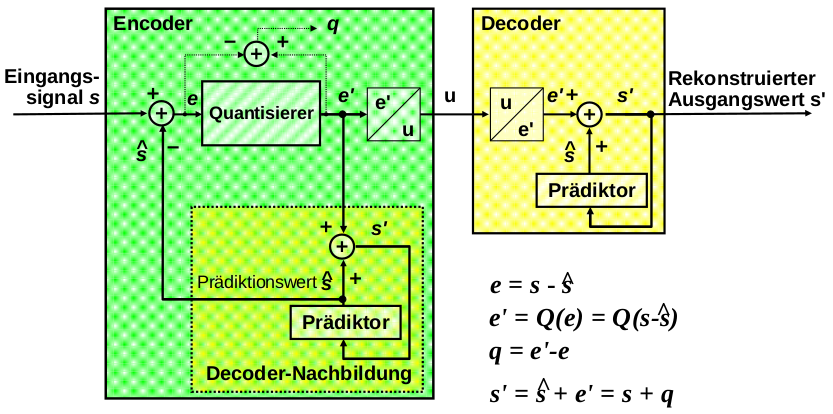
\includegraphics[width=0.8\textwidth]{dpcm}

\subsection*{WHT}

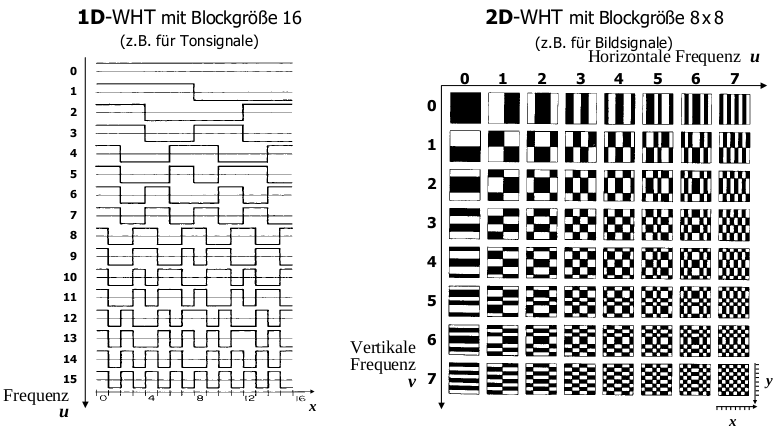
\includegraphics[width=0.8\textwidth]{wht}

\subsection*{$2 \times 2$-WHT-Hintransformation}
\[
    F(u, v) = \frac{1}{2} \sum_{x=0}^{1} \sum_{y=0}^{1} f(x, y) \cdot {(-1)}^{x \cdot u + y \cdot v}
        \quad \mbox{ für } u = 0, 1 \mbox{ und } v = 0, 1
\]

\subsection*{$2 \times 2$-WHT-Rücktransformation}
\[
    f(x, y) = \frac{1}{2} \sum_{u=0}^{1} \sum_{v=0}^{1} F(u, v) \cdot {(-1)}^{x \cdot u + y \cdot v}
        \quad \mbox{ für } x = 0, 1 \mbox{ und } y = 0, 1
\]

\subsection*{DCT}

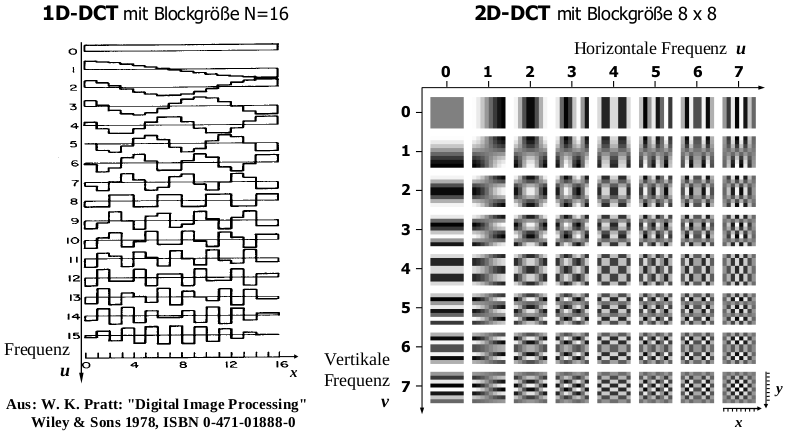
\includegraphics[width=0.8\textwidth]{dct} \\
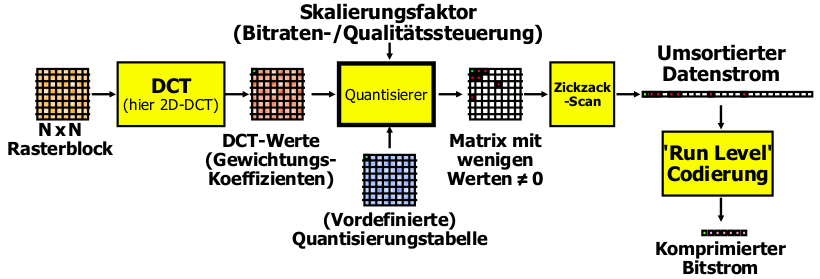
\includegraphics[width=0.8\textwidth]{dct_block}

\subsection*{1D-DCT-Hintransformation}
\[
F(u) = \frac{C(u)}{\sqrt{N}}
    \cdot \sum_{x=0}^{N-1} \bigg[ f(x)
    \cdot \cos{\frac{(2x+1) \cdot u \cdot \pi{}}{2N}}
    \bigg] \mbox{  für } u=0,1,\ldots,N-1
\]
    
\[
    C(u) = \begin{cases}
        1 & \text{für } u=0\\
        \sqrt{2} & \text{sonst}
    \end{cases}
\]

\subsection*{1D-DCT-Rücktransformation}
\[
    f(x) = \sum_{u=0}^{N-1} \bigg[ \frac{C(u)}{\sqrt{N}}
    \cdot F(u)
    \cdot \cos{\frac{(2x+1) \cdot u \cdot \pi{}}{2N}}
    \bigg] \quad \mbox{ für } x=0,1,\ldots,N-1
\]
    
\[
    C(u) = \begin{cases}
        1 & \text{für } u=0\\
        \sqrt{2} & \text{sonst}
    \end{cases}
\]

\subsection*{2D-DCT-Hintransformation}
\[
    F(u, v) = \frac{2}{N} C(u) C(v) \sum_{x=0}^{N-1} \sum_{y=0}^{N-1} \bigg[ f(x, y) \cdot 
    \cos \frac{(2x + 1) \cdot u \cdot \pi}{2 N} \cdot \cos \frac{(2y + 1) \cdot v \cdot \pi}{2 N} \bigg]
\]
    
\[
    C(u) = \begin{cases}
        \frac{1}{\sqrt{2}} & \text{für } u=0\\
        1 & \text{sonst}
    \end{cases}
\]

\subsection*{2D-DCT-Rücktransformation}
\[
    f(x, y) = \frac{2}{N} \sum_{x=0}^{N-1} \sum_{y=0}^{N-1} \bigg[ C(u) C(v) F(u, v) \cdot 
    \cos \frac{(2x + 1) \cdot u \cdot \pi}{2 N} \cdot \cos \frac{(2y + 1) \cdot v \cdot \pi}{2 N} \bigg]
\]
    
\[
    C(u) = \begin{cases}
        \frac{1}{\sqrt{2}} & \text{für } u=0\\
        1 & \text{sonst}
    \end{cases}
\]

\subsection*{JPEG}

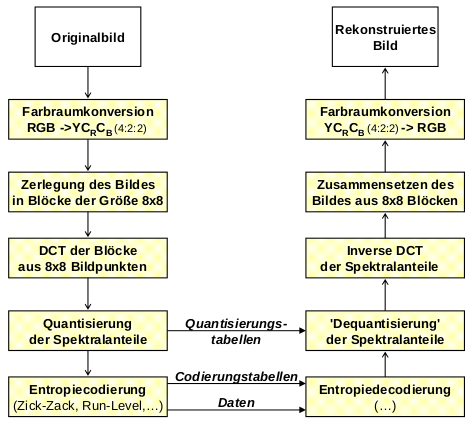
\includegraphics[width=0.6\textwidth]{jpeg}
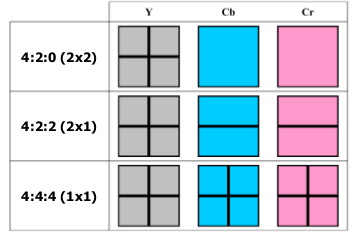
\includegraphics[width=0.35\textwidth]{color_subsampling}

\subsection*{DV}

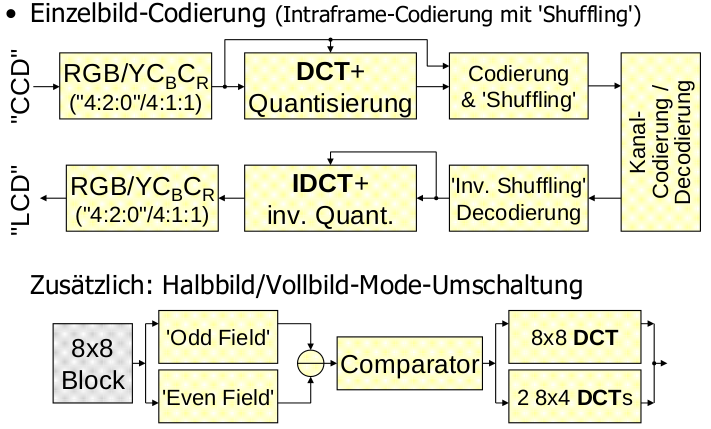
\includegraphics[width=0.8\textwidth]{dv}

\subsection*{MPEG}

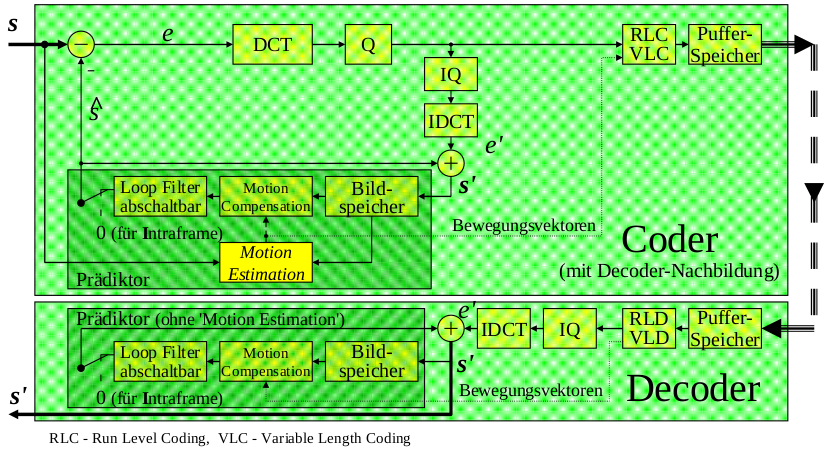
\includegraphics[width=0.8\textwidth]{mpeg}
